\chapter{Results and Interpretation}

Through the extensive procedures outlined in the previous chapter, a set of final results can be provided. Here, the event distributions versus $M_{\gamma^*},\ x_F,\ p_T,\ x_1,$ and $\cos\theta$ are presented. Finally, the per-nucleon cross section ratios are shown for $\sigma^C/\sigma^D$, $\sigma^{Fe}/\sigma^D$, and $\sigma^W/\sigma^D$, along with a comparison of these ratios to previous results and some interpretation of the findings.

\section{Drell-Yan Event Distributions}

The following kinematic distributions represent the acceptance of the SeaQuest dimuon spectrometer. By measuring the momenta ($p_{\mu}$) of the muon tracks at the vertex position, the quantities of invariant mass ($M_{\gamma^*}$), $x_F$, and $p_T$ of the virtual photon can be calculated.
\begin{eqnarray}
p_\mu & = & (p_x, p_y, p_z) \\
E_{\mu^+\mu^-} & = & \sqrt{|p_{\mu^+}|^2 + |p_{\mu^-}|^2} \\
P_{\mu^+\mu^-} & = & p_{\mu^+} + p_{\mu^-} \\
p_T & = & \sqrt{(p_{\mu^+}^x + p_{\mu^+}^x)^2 + (p_{\mu^+}^y + p_{\mu^+}^y )^2} \\
p_z & = & p_{\mu^+}^z + p_{\mu^+}^z \\
M_{\gamma^*} & = & \sqrt{E_{\mu^+\mu^-}^2 - |P_{\mu^+\mu^-}^2|} \\
x_F & = & \frac{p_{\mu^+}^z + p_{\mu^+}^z }{\sqrt{s}/2 (1-M^2_{\gamma^*}/s)} \approx 2(p_{\mu^+}^z + p_{\mu^+}^z)/\sqrt{s} \\
\end{eqnarray}
From these, $x_1$ and $x_2$ can be derived according to Eqs.~\ref{eq:x1-x2-tau}.

\begin{figure}
	\centering
	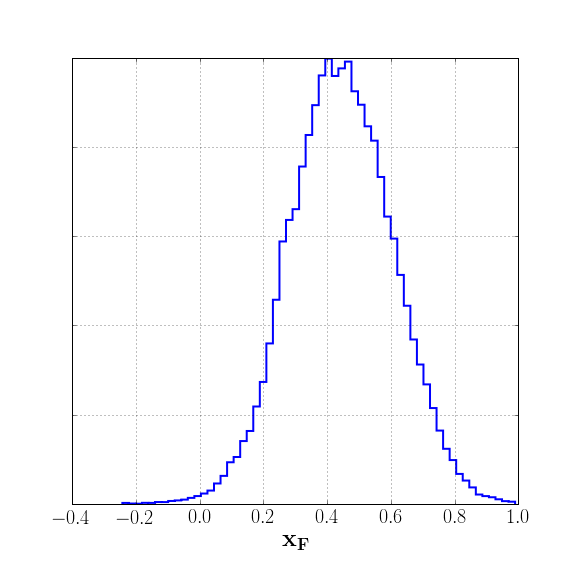
\includegraphics[width=0.48\textwidth]{figures/results/xF-dist.png} \hfill
	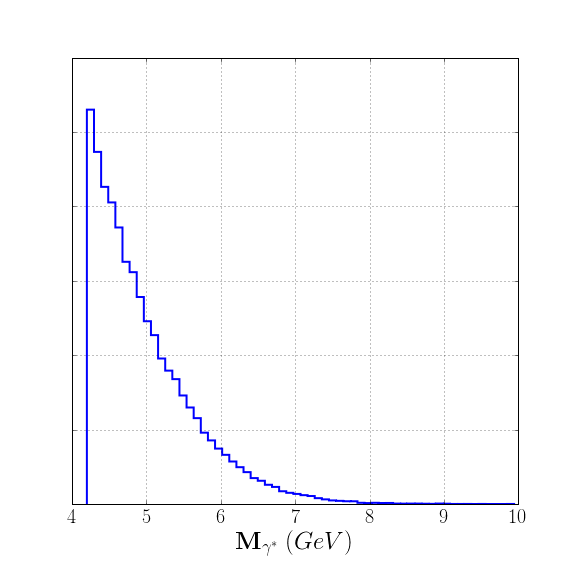
\includegraphics[width=0.48\textwidth]{figures/results/mass-dist.png}    
	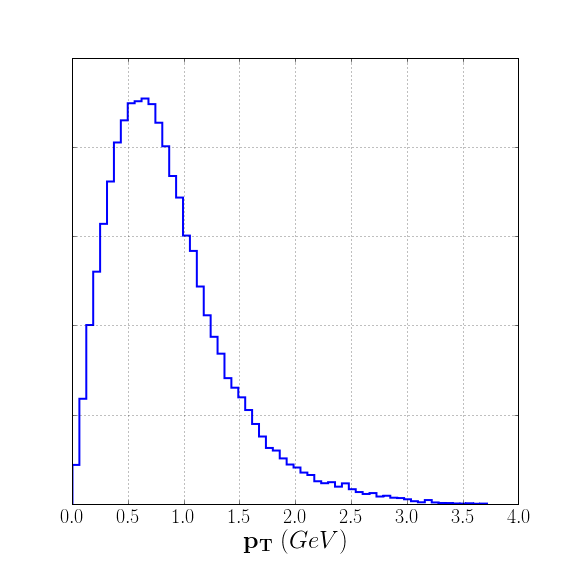
\includegraphics[width=0.48\textwidth]{figures/results/pt-dist.png} \hfill
	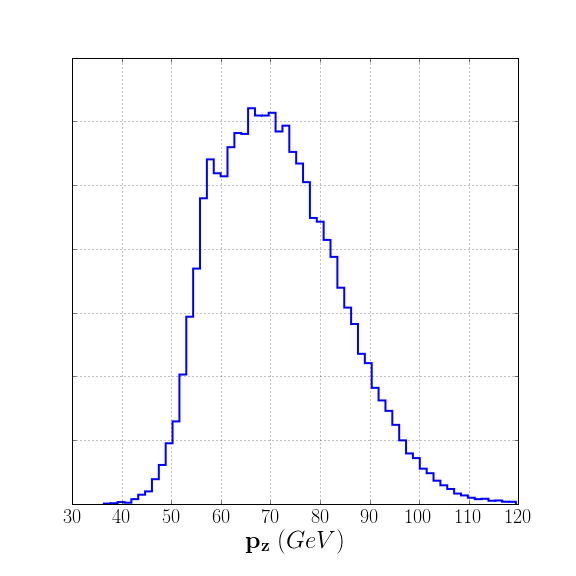
\includegraphics[width=0.48\textwidth]{figures/results/pz-dist.png} \\
	\caption{Event distributions for all combined data versus dimuon kinematic variables $x_F, M_{\gamma^*}, p_T,$ and $p_z$}
	\label{fig:event-dist1}
\end{figure}

\begin{figure}
	\centering
	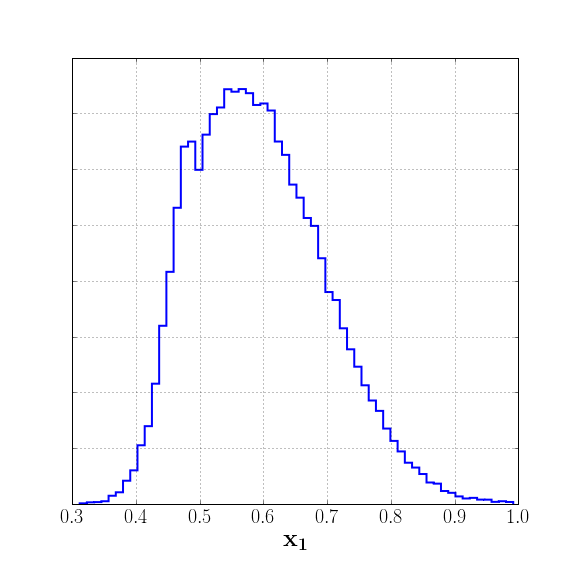
\includegraphics[width=0.48\textwidth]{figures/results/x1-dist.png} \hfill
	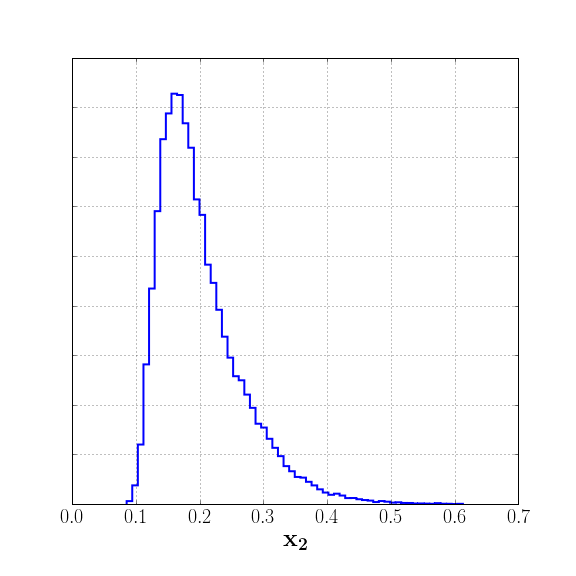
\includegraphics[width=0.48\textwidth]{figures/results/x2-dist.png} \\
	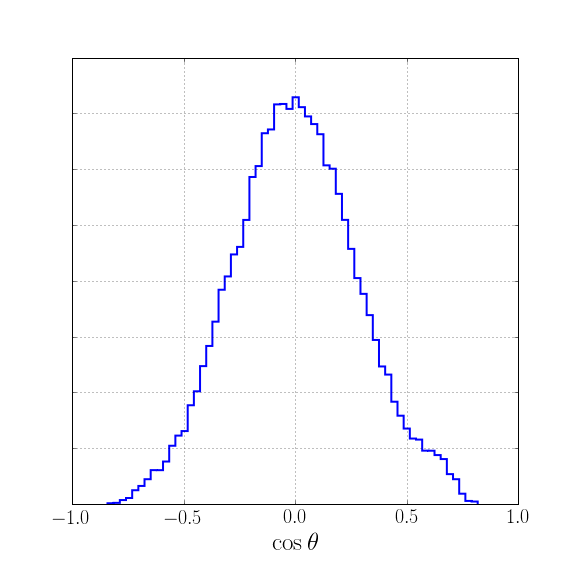
\includegraphics[width=0.48\textwidth]{figures/results/costh-dist.png}
	\caption{Event distributions for all combined data versus quark kinematic variables $x_1, x_2,$ and the cosine of the polar decay angle, $\theta_\mu$}
	\label{fig:event-dist2}
\end{figure}

\begin{sidewaystable}
	\centering
	\ra{1.3}
	\caption*{\textbf{Mean Kinematics}}
	\begin{tabular}{lrrrrrrrrrrrr}
		\toprule
		{} &    $\langle x_1 \rangle$ &    $\langle x_2\rangle$ &   $\langle M_{\gamma^*}\rangle$ &     $\langle x_F\rangle$ &  $\langle \cos\theta_\mu\rangle$ &    $\langle \phi_\mu\rangle$ &     $\langle p_z\rangle$ &    $\langle p_T\rangle$ &     $\langle p_z^+\rangle$ &    $\langle p_z^-\rangle$  &    $\langle p_T^+\rangle$ &   $\langle p_T^-\rangle$  \\
		$x_2$-bin            &        &        &   (GeV)     &        &        &        &     (GeV)    &   (GeV)     &    (GeV)     &   (GeV)      &   (GeV)     &   (GeV)     \\
		\midrule
		(0.1, 0.13]   &  0.746 &  0.120 &  4.378 &  0.690 &  0.011 &  0.043 &  90.145 &  0.737 &  45.815 &  44.329 &  2.124 &  2.112 \\
		\rowcol (0.13, 0.16]  &  0.650 &  0.146 &  4.516 &  0.559 & -0.005 & -0.030 &  78.487 &  0.762 &  39.415 &  39.079 &  2.224 &  2.186 \\
		(0.16, 0.195] &  0.592 &  0.177 &  4.751 &  0.467 & -0.011 & -0.008 &  71.473 &  0.805 &  35.833 &  35.641 &  2.365 &  2.305 \\
		\rowcol (0.195, 0.24] &  0.567 &  0.215 &  5.143 &  0.404 & -0.009 &  0.008 &  68.394 &  0.841 &  34.344 &  34.015 &  2.562 &  2.500 \\
		(0.24, 0.29]  &  0.557 &  0.262 &  5.626 &  0.348 & -0.007 &  0.008 &  67.097 &  0.900 &  33.728 &  33.349 &  2.800 &  2.726 \\
		\rowcol (0.29, 0.35]  &  0.543 &  0.314 &  6.079 &  0.280 & -0.021 &  0.038 &  65.423 &  1.008 &  32.313 &  33.088 &  3.013 &  2.941 \\
		(0.35, 0.45]  &  0.535 &  0.386 &  6.713 &  0.191 & -0.005 &  0.024 &  64.301 &  0.994 &  32.014 &  32.282 &  3.319 &  3.304 \\
		\rowcol (0.45, 0.58]  &  0.512 &  0.485 &  7.331 &  0.040 & -0.019 & -0.220 &  61.508 &  1.086 &  31.295 &  30.323 &  3.715 &  3.626 \\
		\bottomrule
		\textbf{Combined:} & 0.601 &  0.201 &  5.012 &  0.453 & -0.002 & 0.000 & 72.553 &  0.865 &  36.444 &  36.109 &  2.472 & 2.441 \\
	\end{tabular}
	\caption{The mean dimuon kinematics in each bin of $x_2$. These should be considered to be appro/ximate, as they are
		calculated as a weighted average from the data set when corrected for rate dependence in $x_2$.}
	\label{tab:mean-kin-x2}
\end{sidewaystable}

The distributions of the dimuon kinematic quantities $x_F, M_{\gamma^*}, p_T$, and $p_z$ can be found in Figure~\ref{fig:event-dist1} while the quark quantities $x_1, x_2,$ and $\cos\theta_\mu$ can be found in Figure~\ref{fig:event-dist2}. As can be seen from the distributions, the SeaQuest experiment studies muons with an invariant mass between 4.2 and \unit[10]{GeV} (the range between the $\psi^\prime$ and the $\Upsilon$), and the acceptance measures mostly forward-moving ($x_F>0$) muon pairs with longitudinal momentum ($p_z$) greater than \unit[40]{GeV} in the lab frame. The acceptance of $p_T$ of the muon pair is limited to \unit[3]{GeV}. It is worth noting that, as can be seen from the $\cos\theta_\mu$ distribution, there is certainly contamination evident at the tails of the distribution, primarily in the positive $\cos\theta$ region. This is one of the key clues that SeaQuest has a problem with \emph{combinatoric} background, or reconstructed muon pairs that arise from uncorrelated muons produced in the target or beam dump.

The beam quarks participating in the Drell-Yan process can have a fractional momentum $x_1$ ranging from around 0.35 to 0.9 with the distribution peaking at 0.57 and having a mean value of $\langle x_1 \rangle = 0.6$. The target antiquark participating in the interaction can possess a fractional momentum $x_2$ ranging from 0.1 to 0.5, with the distribution peaking at around 0.16 and having a mean value of $\langle x_2 \rangle = 0.2$. A table of the total mean kinematics and also the mean kinematics for each $x_2$ bin can be found in Table~\ref{tab:mean-kin-x2}.




\section{The A-Dependence of the Drell-Yan Process}

The ratio for $R_{DY}^{A/D}$ are presented here, where the ratio is defined Eq.~\ref{eq:dy-ratio} and \ref{eq:targ-to-targ-norm}. Results are presented for the nuclear-to-deuterium ratios for carbon, iron, and tungsten. The results are presented in the following order:
\begin{itemize}
	\item The ratio versus dimuon kinematics $M_{\gamma^*}, x_F,$ and $p_T$
	\item The ratio versus quark kinematics $x_1, x_2,$ and $\cos\theta_\mu$
	\item The ratio versus $x_2$ for the three roadsets analyzed
	\item The ratio versus $x_2$ for two bins of $p_T$, two bins of $x_1$, and two bins of $M_{\gamma^*}$ (two $Q^2$ intervals)
	\item The integrated ratio versus mass number $A$.
\end{itemize}
But before results are presented, a total systematic uncertainty will be estimated to consider when evaluating the results.

\subsection{Systematic Uncertainties}

The types of systematic uncertainties considered here are the following:
\begin{enumerate}
	\item Liquid deuterium contamination
	\item kEfficiency curve fit uncertainty
	\item Empty target curve fit uncertainty
	\item Empty target normalization constant uncertainty
	\item Remaining rate dependence uncertainty.
\end{enumerate}
These factors were each independently varied from their nominal values to $\pm1\sigma$, and the final ratio measurement was evaluated for each of the three settings. The percentage change between of the final result is what is quoted as the systematic uncertainty for that particular factor. With each uncertainty evaluated, the upper and lower bounds of asymmetric uncertainties were combined in quadrature.

In dealing with the asymmetric uncertainty in the deuterium contamination, it was found to have a uniform effect across targets and binning of $+2\% / -1.4\%$. The kEfficiency exponential fit uncertainty has a target dependence since the fit parameter was evaluated for different nuclear targets. These uncertainties are shown in Table~\ref{tab:sys-keff}, and in general are around $\pm2\%$. The Empty target curve fit parameter uncertainty had little effect and led to $\pm0.1-0.7\%$ variation in the ratios. The uncertainty in the normalization constant, B, of the empty target background subtraction also propagated a small variation of $\pm0.1-0.7\%$. The remaining rate dependence was previously evaluated to be 1.07\% when it was defined.

Without any approximation, the calculated asymmetric systematic uncertainties were combined in quadrature (independently for the upper and lower intervals) to yield the total estimation, as seen in Table~\ref{tab:total-sys}. To a good approximation, it can be stated that the systematic uncertainty of a nuclear cross section ratio measurement at SeaQuest due to the above-described sources can, to a good approximation, be considered to be $\pm3\%$, with it being slightly higher in the case of tungsten and slightly lower in the case of carbon.

\begin{table}
	\centering
	\begin{tabular}{lrrrrrr}
		\toprule
		$x_2-$bin &   C/D- &   C/D+ &  Fe/D- &  Fe/D+ &   W/D- &   W/D+ \\
		\midrule
		(0.1, 0.13]   & -0.010 &  0.011 & -0.018 &  0.019 & -0.024 &  0.025 \\
		(0.13, 0.16]  & -0.016 &  0.016 & -0.011 &  0.011 & -0.023 &  0.023 \\
		(0.16, 0.195] & -0.017 &  0.018 & -0.025 &  0.026 & -0.027 &  0.028 \\
		(0.195, 0.24] & -0.020 &  0.020 & -0.017 &  0.018 & -0.024 &  0.025 \\
		(0.24, 0.29]  & -0.013 &  0.014 & -0.017 &  0.018 & -0.018 &  0.018 \\
		(0.29, 0.35]  & -0.015 &  0.015 & -0.018 &  0.018 & -0.023 &  0.023 \\
		(0.35, 0.45]  & -0.009 &  0.009 & -0.022 &  0.023 & -0.009 &  0.009 \\
		(0.45, 0.58]  &  -0.005 & 0.004 & -0.016 &  0.016 & -0.012 &  0.012 \\
		\bottomrule
	\end{tabular}
	\caption{Systematic error arising from the uncertainty in the kEfficiency exponential fit parameter.}
	\label{tab:sys-keff}
\end{table}

\begin{table}
	\centering
	\caption*{Fractional Systematic Uncertainties}
	\begin{tabular}{lrrrrrr}
		\toprule
		$x_2-$bin &   C/D- &   C/D+ &  Fe/D- &  Fe/D+ &   W/D- &   W/D+ \\
		\midrule
		(0.1, 0.13]   &  0.021 &  0.025 &  0.028 &  0.030 &  0.032 &  0.035 \\
		(0.13, 0.16]  &  0.023 &  0.028 &  0.023 &  0.027 &  0.031 &  0.034 \\
		(0.16, 0.195] &  0.025 &  0.029 &  0.032 &  0.035 &  0.034 &  0.037 \\
		(0.195, 0.24] &  0.026 &  0.030 &  0.027 &  0.030 &  0.032 &  0.035 \\
		(0.24, 0.29]  &  0.022 &  0.026 &  0.027 &  0.030 &  0.028 &  0.031 \\
		(0.29, 0.35]  &  0.023 &  0.028 &  0.029 &  0.030 &  0.031 &  0.034 \\
		(0.35, 0.45]  &  0.019 &  0.026 &  0.030 &  0.034 &  0.022 &  0.027 \\
		(0.45, 0.58]  &  0.022 &  0.038 &  0.024 &  0.029 &  0.022 &  0.030 \\
		\bottomrule
	\end{tabular}
	\caption{The total estimated \emph{fractional} systematic uncertainty for the ratio measurements versus $x_2$.}
	\label{tab:total-sys}
\end{table}

\subsection{$M_{\gamma^*}, x_F,$ and $p_T$ Dependence}

Shown in Figure~\ref{fig:mass-emc} is the nuclear cross section ratio as a function of invariant mass for the three heavy nuclei. While dimuons are accepted up to \unit[10]{GeV}, there is little-to-no signal that passes all cuts above \unit[7.5]{GeV}. Figure~\ref{fig:xf-emc} shows the ratio's dependence on $x_F$, where an enhancement can be seen below $x_F<0.5$ and a depletion in the ratio value can be seen above $x_F>0.5$. Figure~\ref{fig:pt-emc} shows the ratio as a function of $p_T$, where there is a trend of a depletion in the ratio for low $p_T<\unit[0.5]{GeV}$ and an excess beyond that point. Lastly, there is the ratio versus the longitudinal momentum, $p_z$, in Figure~\ref{fig:pz-emc}, where no significant trend in behavior is observed.

\begin{sidewaysfigure}
	\centering
	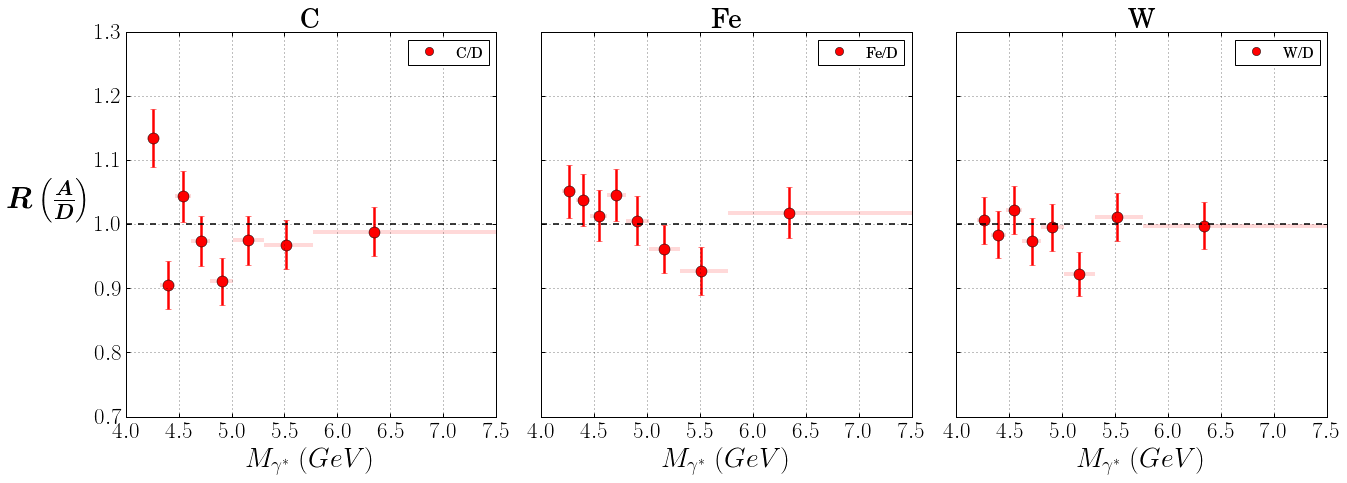
\includegraphics[width=0.85\textwidth]{figures/results/mass-emc.png}
	\caption{The measured Drell-Yan per-nucleon cross section ratio against invariant dimuon mass. Only statistical uncertainty is shown.}
	\label{fig:mass-emc}
	\vspace{1cm}
	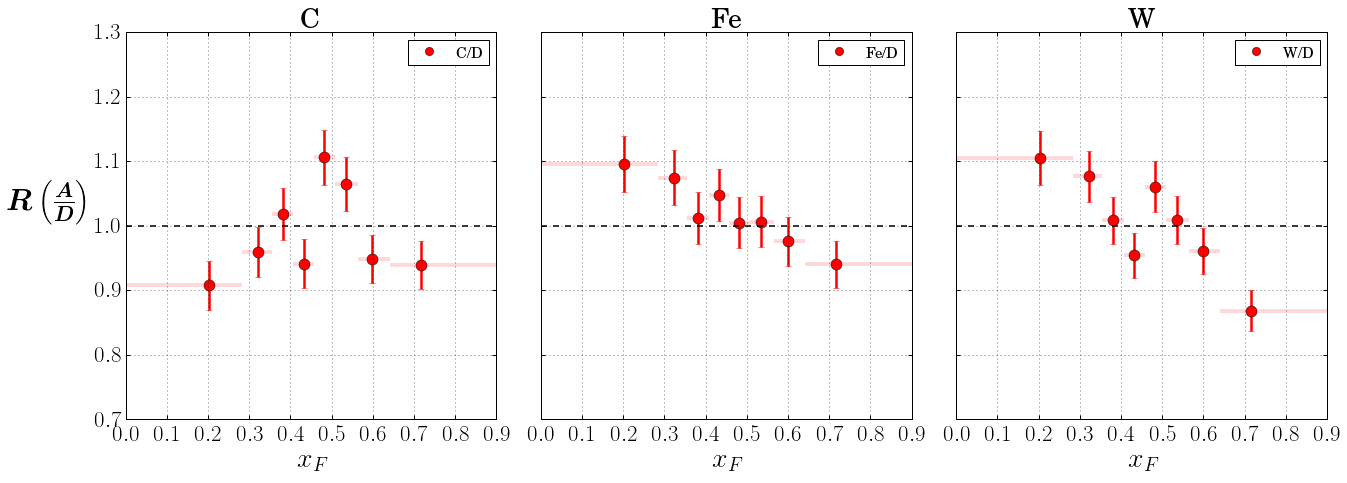
\includegraphics[width=0.85\textwidth]{figures/results/xF-emc.png}
	\caption{The measured Drell-Yan per-nucleon cross section ratio against dimuon Feynman-$x$. Only statistical uncertainty is shown.}
	\label{fig:xf-emc}
\end{sidewaysfigure}

\begin{sidewaysfigure}
	\centering
	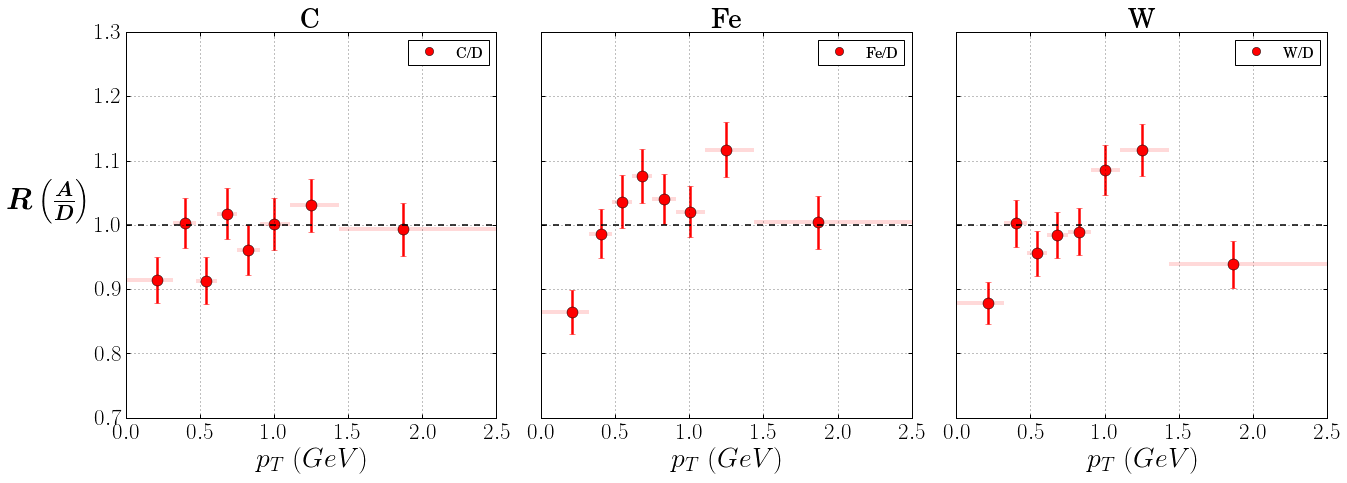
\includegraphics[width=0.85\textwidth]{figures/results/pT-emc.png}
	\caption{The measured Drell-Yan per-nucleon cross section ratio versus transverse momentum of the muon pair. Only statistical uncertainty is shown.}
	\label{fig:pt-emc}
	\vspace{1cm}
	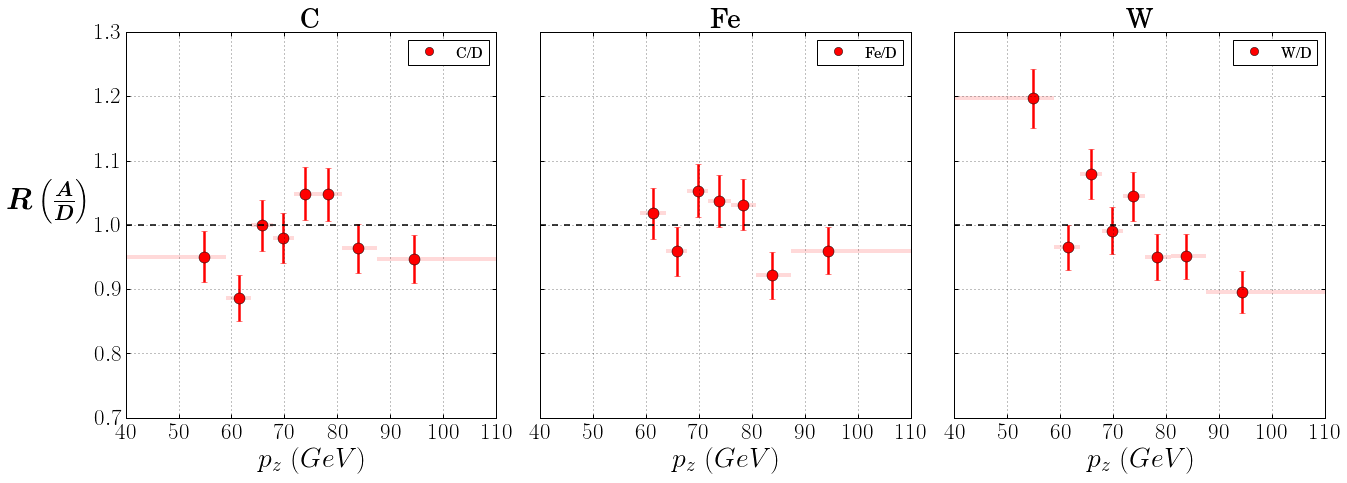
\includegraphics[width=0.85\textwidth]{figures/results/pz-emc.png}
	\caption{The measured Drell-Yan per-nucleon cross section ratio versus longitudinal momentum of the muon pair. Only statistical uncertainty is shown.}
	\label{fig:pz-emc}
\end{sidewaysfigure}

\subsection{$x_1, x_2,$ and $\cos\theta_\mu$ Dependence}

The quark variables $x_1$ and $x_2$, which are the momentum fractions of the beam and target hadrons carried by the interacting quarks, respectively. Figure~\ref{fig:xB-emc} shows the values of $R_{DY}(A/D)$ as a function of $x_1$ for each target. Figure~\ref{fig:xT-emc} shows the values of the ratio $R_{DY}(A/D)$ as a function of $x_2$, which is the main focus of this analysis. This plot is zoomed out to show an anomalously low point for the carbon target at $(x_2, R_{DY})=(0.48, 0.39)$. The same figure zoomed in to match the rest of the plots can be found in Figure~\ref{fig:xT-emc-zoomed}. Across the three targets, a depletion is observed at $x_2<0.15$. Elsewhere, there appears to be a small excess in the $0.15<x_2<0.25$ for iron and tungsten. This depletion appears to be approximately an 8\% depletion for all targets at $x_2=0.12$. A tabulation of the data from this plot can be found in Table~\ref{tab:emc-data-x2}, including estimated asymmetric systematic uncertainties.

This data for this is also broken up into the three roadsets in Figure~\ref{fig:emc-roadset} and into two bins of $p_T$ in Figure~\ref{fig:xt-pt-emc}. It is clear from the roadset comparison that there is considerable disagreement at higher $x_2>0.25$, but the tungsten data seems to agree up to $x_2=0.35$. When binned in high and low bins of $p_T$, there seems to be a systematic excess in the heavier nuclear component of the ratio for high-$p_T$ events ($p_T>\unit[0.6]{GeV}$).

\begin{sidewaysfigure}
	\centering
	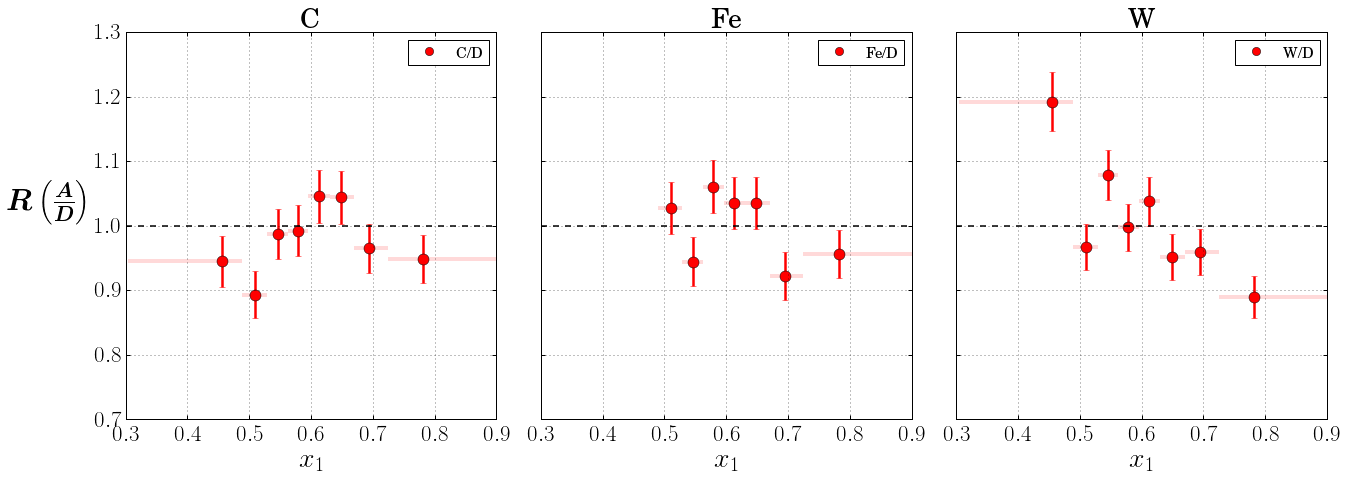
\includegraphics[width=0.85\textwidth]{figures/results/xB-emc.png}
	\caption{The measured Drell-Yan per-nucleon cross section ratio versus fractional momentum quantity, $x_1$. Only statistical uncertainty is shown.}
	\label{fig:xB-emc}
	\vspace{1cm}
	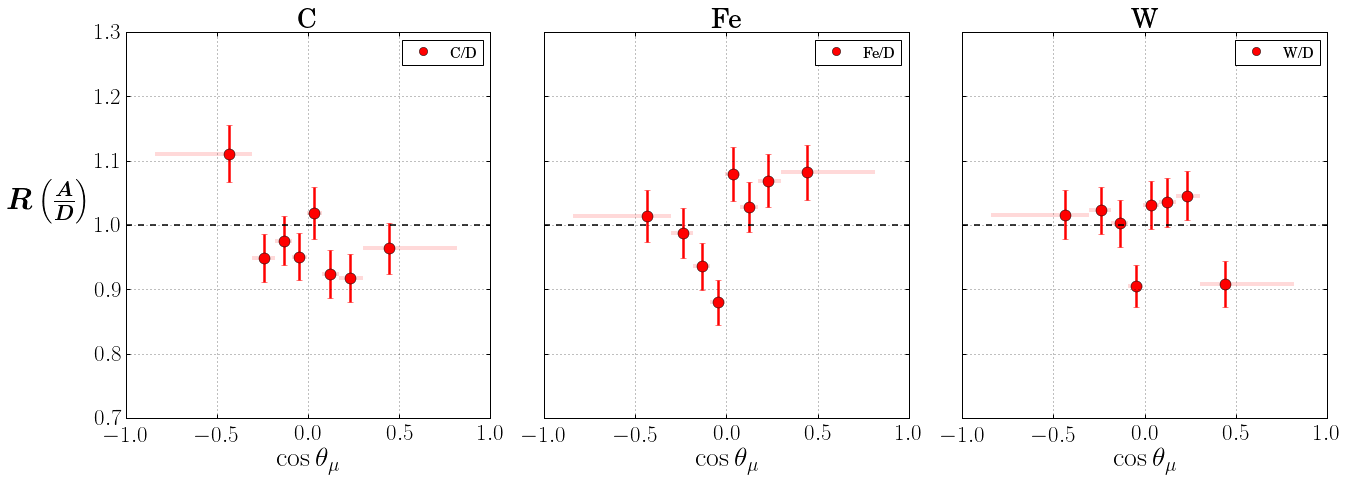
\includegraphics[width=0.85\textwidth]{figures/results/costh-emc.png}
	\caption{The measured Drell-Yan per-nucleon cross section ratio versus the cosine of the polar muon production angle, $\theta_\mu$. Only statistical uncertainty is shown.}
	\label{fig:costh-emc}
\end{sidewaysfigure}
\begin{sidewaysfigure}
	\centering
	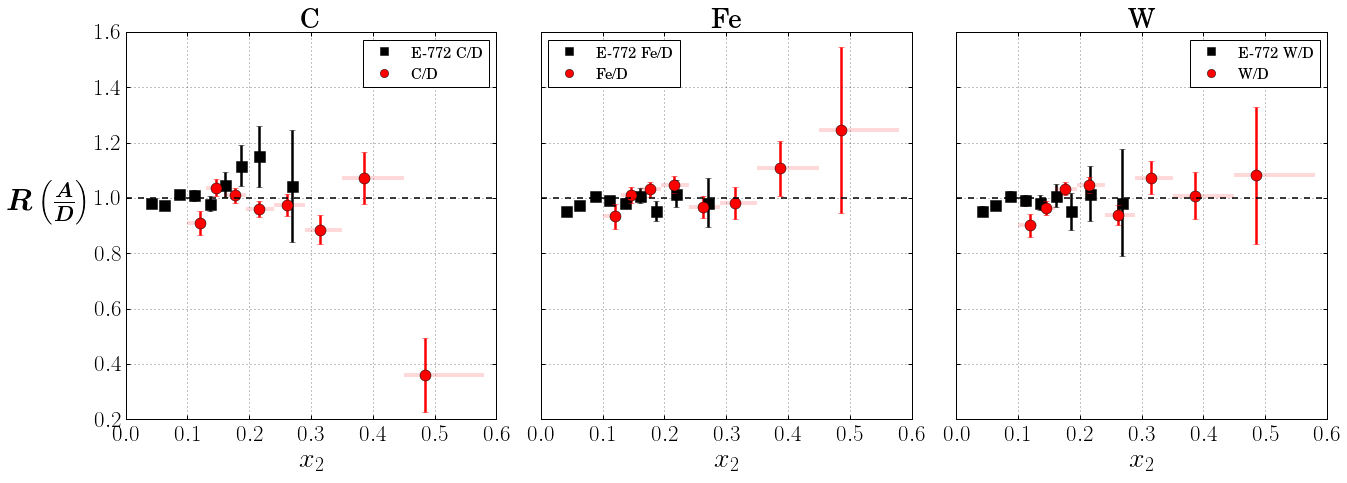
\includegraphics[width=0.85\textwidth]{figures/results/xT-emc.png}
	\caption{The measured Drell-Yan per-nucleon cross section ratio versus fractional momentum quantity, $x_2$. Only statistical uncertainty is shown. Overlaid is the data from the E-772 experiment.}
	\label{fig:xT-emc}
	\vspace{1cm}
	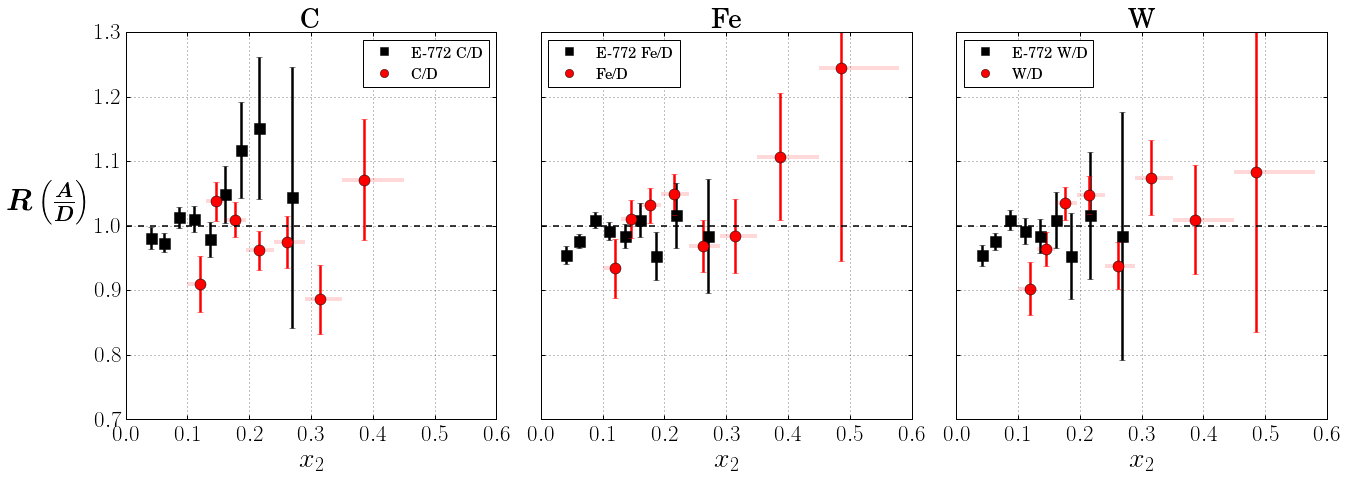
\includegraphics[width=0.85\textwidth]{figures/results/xT-emc-zoom.png}
	\caption{The same plot, but zoomed into R=[0.7, 1.2] for closer comparison with E-772 data.}
	\label{fig:xT-emc-zoomed}
\end{sidewaysfigure}

\begin{sidewaysfigure}
	\centering
	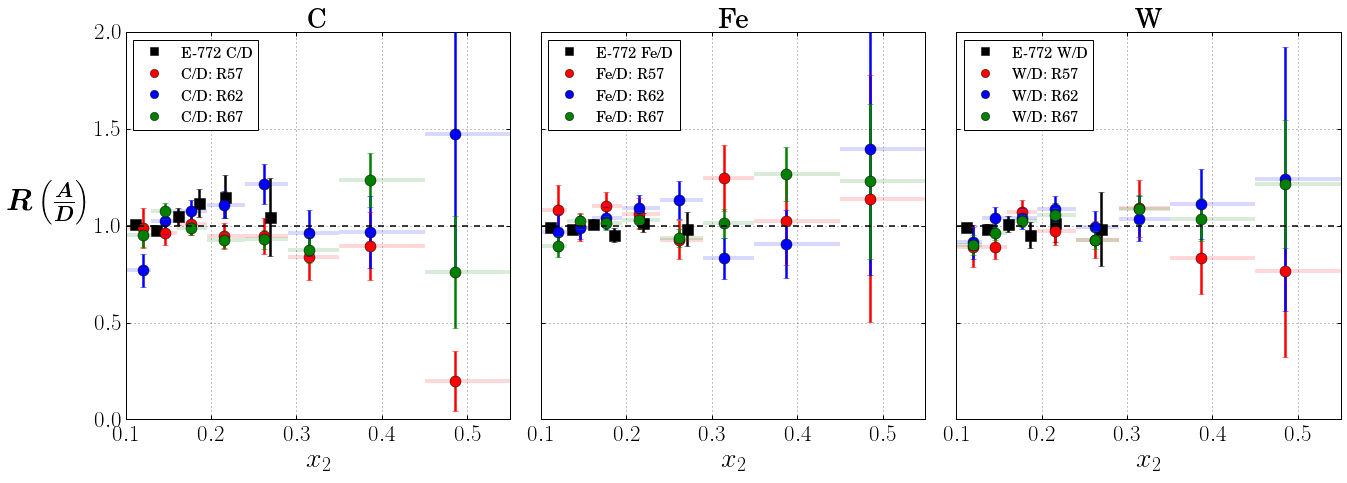
\includegraphics[width=0.85\textwidth]{figures/results/xT-emc-roadset.png}
	\caption{The measurement of $R_{DY}$ for the three roadsets. Their results are combined to render the values found in Figure~\ref{fig:xT-emc}.}
	\label{fig:emc-roadset}
	\vspace{1cm}
	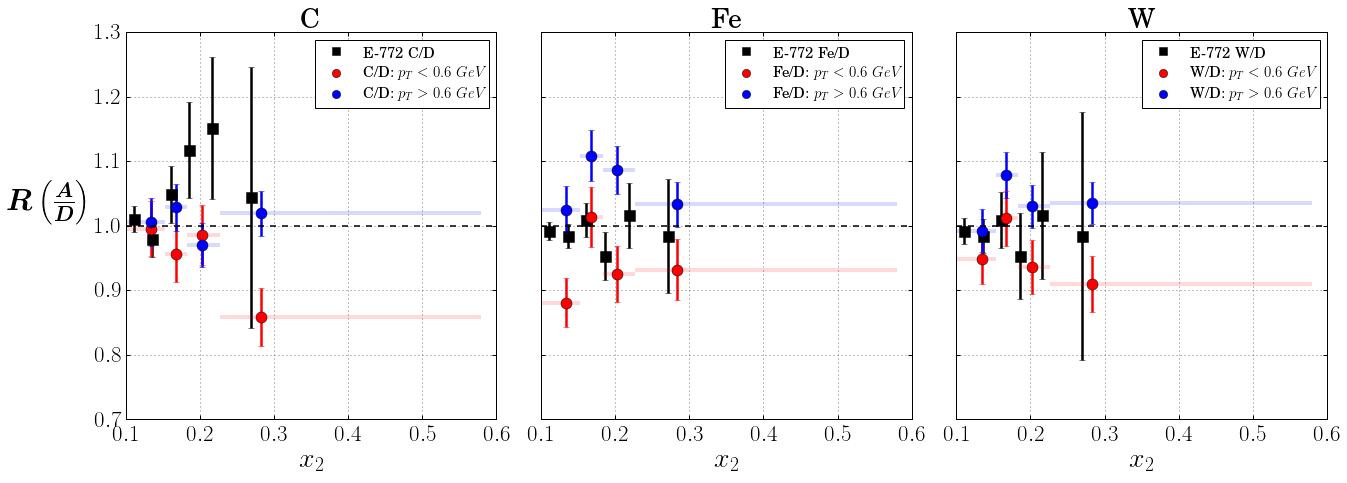
\includegraphics[width=0.85\textwidth]{figures/results/xT-emc-pT.png}
	\caption{The measured Drell-Yan per-nucleon cross section ratio versus fractional momentum quantity, $x_2$, grouped into ``high'' $p_T$ and ``low'' $p_T$. Only statistical uncertainty is shown.}
	\label{fig:xt-pt-emc}
\end{sidewaysfigure}

\begin{table}
	\centering
	\begin{tabular}{@{}llrrlrrlrr@{}}
		\toprule
		$\langle x_2 \rangle$  &     C/D &     sys.- &     sys.+ &           Fe/D &    sys.- &   sys.+ &            W/D &     sys.- &     sys.+ \\
		\midrule
		0.12 &    0.91$\pm$0.04 &  0.019 &  0.022 &    0.93$\pm$0.05 &  0.026 &  0.028 &    0.90$\pm$0.04 &  0.029 &  0.032 \\
		0.15 &  1.038$\pm$0.030 &  0.024 &  0.029 &  1.011$\pm$0.029 &  0.024 &  0.027 &  0.964$\pm$0.026 &  0.030 &  0.033 \\
		0.18 &  1.010$\pm$0.027 &  0.025 &  0.029 &  1.032$\pm$0.027 &  0.034 &  0.036 &  1.035$\pm$0.025 &  0.035 &  0.038 \\
		0.22 &  0.962$\pm$0.030 &  0.025 &  0.029 &  1.049$\pm$0.031 &  0.028 &  0.031 &  1.048$\pm$0.029 &  0.034 &  0.037 \\
		0.26 &   0.98$\pm$0.04 &  0.022 &  0.026 &    0.97$\pm$0.04 &  0.026 &  0.029 &    0.94$\pm$0.04 &  0.026 &  0.029 \\
		0.31 &   0.89$\pm$0.05 &  0.021 &  0.025 &    0.98$\pm$0.06 &  0.029 &  0.030 &    1.07$\pm$0.06 &  0.034 &  0.037 \\
		0.39 &   1.07$\pm$0.09 &  0.020 &  0.028 &    1.11$\pm$0.10 &  0.033 &  0.037 &    1.01$\pm$0.08 &  0.022 &  0.027 \\
		0.49  &   0.36$\pm$0.13 &  0.008 &  0.014 &    1.24$\pm$0.30 &  0.030 &  0.036 &    1.08$\pm$0.25 &  0.024 &  0.032 \\
		\bottomrule
	\end{tabular}
	\caption{The tabulated data of $R_{DY}(A/D)$ for C/D, Fe/D, and W/D, fully with statistical uncertainty and upper and lower asymmetric systematic uncertainties.}
	\label{tab:emc-data-x2}
\end{table}

\subsection{Integrated Ratio versus A}

Integrating over any existing kinematic dependence, Figure~\ref{fig:int-dy-a} shows the ratio of total yields between $\sigma^C/\sigma^D$, $\sigma^{Fe}/\sigma^D$, and $\sigma^W/\sigma^D$ plotted against the atomic weight $A$. Weights 12.0107, 55.845, and 183.84 were used for carbon, iron, and tungsten respectively. Each data point has approximately a 1.7\% statistical error, with the $\sim3\%$ systematic uncertainty now shown. The ratio of integrated carbon yields to deuterium yields appears to be consistent with unity while iron and tungsten show a very slight enhancement.

\begin{figure}
	\centering
	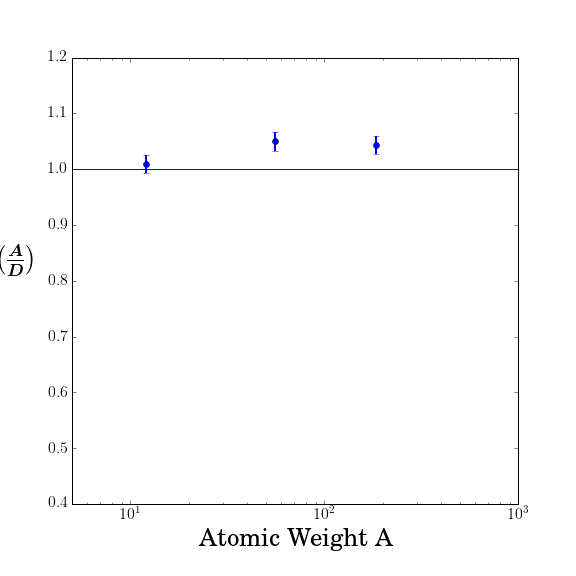
\includegraphics[width=0.5\textwidth]{figures/results/int-DY-A.png}
	\caption{Event distributions for all combined data versus quark kinematic variables $x_1, x_2,$ and the cosine of the polar decay angle, $\theta_\mu$}
	\label{fig:int-dy-a}
\end{figure}

\section{Discussion of $R_{DY}(x_2)$}

As discussed in Section~\ref{sec:dy-emc-sea}, a particularly interesting nuclear cross section ratio is that of DY versus $x_2$. To good approximation, the following should hold:
\begin{equation}
R^{DY}(x_2) \approx \frac{\bar{u}^A(x_2)}{\bar{u}^d(x_2)}.
\end{equation}
Looking at the results in this context, it would appear that when also considering the additional 3\% systematic uncertainty, there seems to be little modification of the sea quark distribution due to nuclear effects.

Here, some topics regarding this measurement are discussed, including a criticism and alternate proposal for calculating ratios and combining separate measurements. This is followed by a comparison with the only other comparable result that exists, E-772. Finally, some of the models that make some predictions regarding the DY nuclear cross section ratio are briefly addressed and discussed.

\subsection{Natural Log of Ratios}

\begin{wrapfigure}{R}{0pt}
	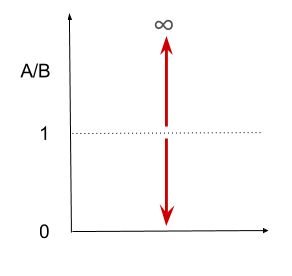
\includegraphics[width=0.3\textwidth]{figures/results/non-log.png} \newline
	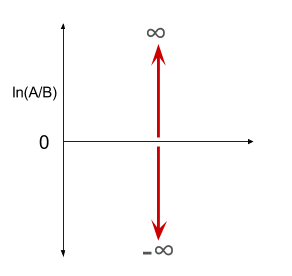
\includegraphics[width=0.3\textwidth]{figures/results/log.png}
	\caption{A depiction of the asymmetric phase space for A/B versus $\ln (A/B)$.}
	\label{fig:log-nolog}
\end{wrapfigure}
It has been recently discussed within the SeaQuest collaboration that perhaps the usual way of measuring, calculating, and visualizing ratios has been historically flawed -- or more flawed than need be. To begin this explanation, consider the simple case of plotting a non-negative ratio of two numbers A and B. In Figure~\ref{fig:log-nolog}, one can see the available phase space for such a value in the case of a direct ratio of A/B and the available phase space for the natural log of the ratio. The natural log representation shows a more desirably symmetric available phase space.

Further, consider the values of A=200 and B=150. If one wished to establish the relation of these two quantities, one might find it desirable that the plotting of A/B yields an opposite yet symmetric result with respect to B/A. Instead, what is seen is a \emph{visually} (but not mathematically) deceiving asymmetric representation. One way shows A/B=$1.3\bar{3}$, and the other shows B/A=0.75. If one were to attempt to characterize an asymmetry in the quantities based upon the \emph{magnitude of the deviation from unity}, then the impression of the magnitude of the asymmetry would change with respect to which quantity one chooses as the numerator and which one chooses for the denominator.

Another hint that a change in representation may be in order is the existence of nonsense error bars for low ratio value measurements. It is possible, though it should not be, in some cases with low statistics, that an error calculated for A/B to measure its nominal value R and uncertainty $\sigma$ to have a lower bound of $R-\sigma < 0$. For a non-negative ratio, this makes no sense, and as such indicates that perhaps this should be handled differently.

The reason for the above is primarily due to uncertainties only being calculated to first order.  By this, I refer to the case that the uncertainty of a function $f(x)$ can be expressed as a Taylor expansion:
\begin{equation}
\Delta f(x) = \sum\limits_i^\infty \frac{d^i f(x)}{dx^i} (\Delta x)^i.
\end{equation}
In the case of the ratio A/B, this contributes \emph{one} term to the ratio uncertainty when considering the variation in A, but infinite terms when considering the variation in B (which are likely completely ignored). When considering the natural log of the ratio, this uncertainty is redistributed in such a way that, even if the series is only calculated to first order, it is done equally to both numerator and denominator.

\begin{figure}
	\centering
	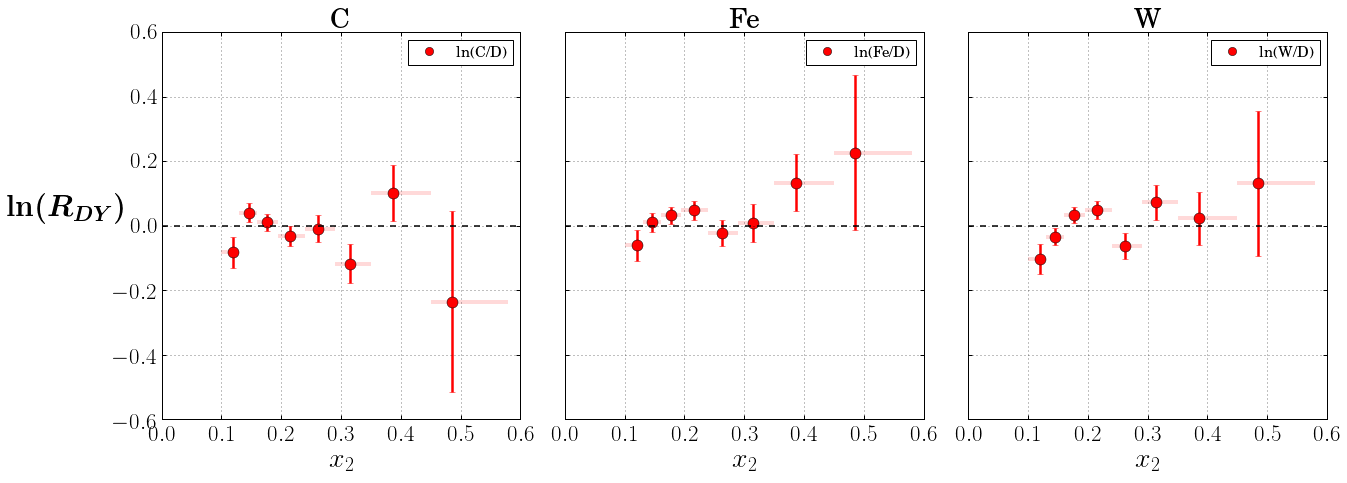
\includegraphics[width=\textwidth]{figures/results/xt-emc-log.png}
	\caption{The combined results of the log of $R_{DY}$ from the three roadsets.}
	\label{fig:xt-emc-log}
\end{figure}

Let us now look at a re-evaluation of the ratio represented in Figure~\ref{fig:xT-emc}. Please make special note of anomalously low value in the highest $x_2$ bin of $\sigma^C/\sigma^D$ and how it appears to be $\sim4\sigma$ away from unity. Now, we re-evaluate the ratio by calculating
\begin{equation}
L_{DY} = \ln(R_{DY} = \ln(Y_A/Y_D) = ln(Y_A) - ln(Y_D),
\end{equation}
where $Y_A$ is the normalized yield for target A, propagating first order uncertainties along the way. Once there, if it is so desired, one can translate directly back from the natural log ratio evaluation to the  bare ratio evaluation by taking the exponential of each data point and \emph{the absolute location of the $1\sigma$ uncertainty boundaries}, not the magnitude of the uncertainties.

In Figure~\ref{fig:xt-emc-log} shows what the combined results look like if the log ratios are calculated. It is difficult to have an intuition for the values of $\ln(R_{DY})$, but here the statistical error bars avoid the possibility of crossing a forbidden boundary. Now, what happens when all the nominal points and upper and lower statistical boundaries are mapped back into $R_{DY}$ values with an exponential function.

Here in Figure~\ref{fig:xt-emc-nonlog}, we see something unexpected -- the anomalously low point for carbon at high $x_2$ that was observed in the original Figure~\ref{fig:xT-emc} is now bumped up significantly from $R_{DY}=0.36$ up to $R_{DY}=0.8$. The tabulated data from this can be found in Table~\ref{tab:log-combined}. \emph{How could this simple transformation have such a drastic effect?}

\begin{figure}
	\centering
	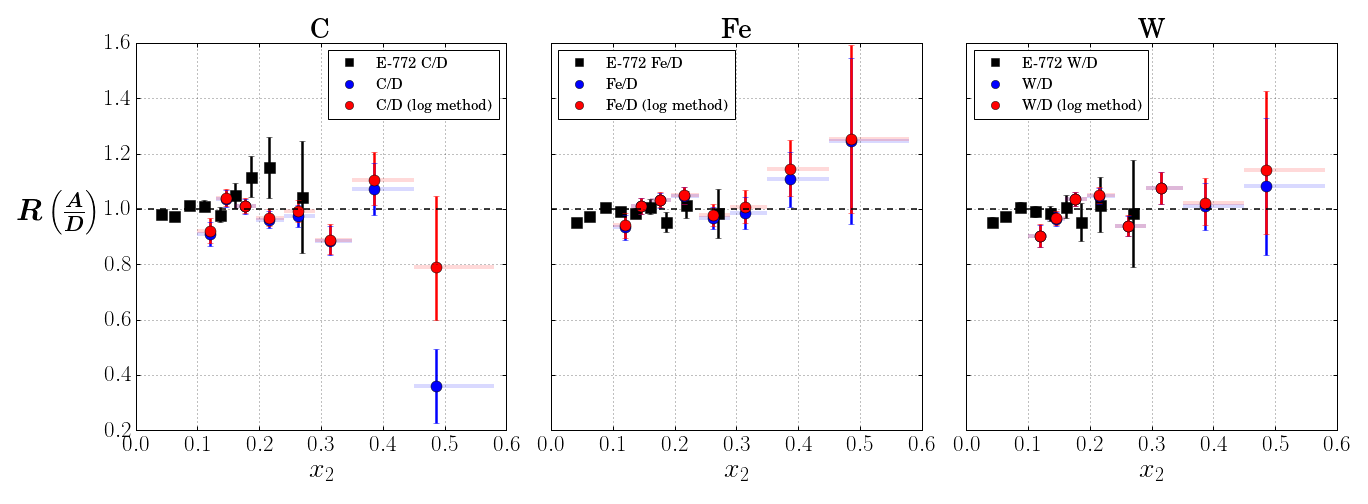
\includegraphics[width=\textwidth]{figures/results/xt-emc-nonlog-vs-old.png}
	\caption{The combined results of the log of $R_{DY}$ transformed back into a plot of $R_{DY}$ by mapping the data points and error bounds with the exponential function.}
	\label{fig:xt-emc-nonlog}
\end{figure}

The answer is bipartate: it lies in (1) the poor estimate in uncertainty of $R_{DY}=Y_A/Y_D$ when the ratio is taken directly, and (2) the way in which different measurements are combined. When a cross section ratio measurement is made for each of the three roadsets ($R_i$), the ratio values are combined ($R_C$) via the following:
\begin{eqnarray}
R_1 & = & Y^A_1/Y^D_1,\ \ R_2 = Y^A_2/Y^D_2, ... \\
& & \nonumber \\
R_C & = & \frac{\sum\limits_i R_i/\sigma_i^2}{\sum\limits_i 1/\sigma_i^2} \\
& & \nonumber \\
\delta R_C & = & \frac{1}{\sqrt{\sum\limits_i 1/\sigma_i^2}}
\end{eqnarray}
The problem arises that when the combined measurement is weighted by the uncertainties, and the uncertainties are poorly defined, then this can really have a substantial effect on where the actual data point ends up.

By transforming to the $R_i \rightarrow L_i = \ln(R_i)$, more appropriate uncertainties can be approximated and used to combine many measurements of $L_i$ into a combined $L_C$ by the method described just above, and then those combined data points and absolute uncertainties are translated back to $R_{DY}$.

At the time of this writing, SeaQuest is actively attempting to re-evaluate the previous results of the ratio measurements made by E-866 to investigate the full extent to which this representation and uncertainty calculation may influence their results. In the E-866 $\sigma^D/\sigma^H$ measurement, there is a \emph{very} similar situation of three data sets being combined, resulting in the highest $x-$bin showing an anomalously depleted value. No model has been fully able to explain this behavior.

\begin{table}
	\centering
	\begin{tabular}{lrrrrrr}
		\toprule
		{} &   C/D- &   C/D+ &  Fe/D- &  Fe/D+ &   W/D- &   W/D+ \\
		\midrule
		(0.1, 0.13]   &  0.878 &  0.967 &  0.897 &  0.987 &  0.862 &  0.944 \\
		(0.13, 0.16]  &  1.011 &  1.072 &  0.982 &  1.041 &  0.941 &  0.994 \\
		(0.16, 0.195] &  0.985 &  1.039 &  1.006 &  1.061 &  1.010 &  1.061 \\
		(0.195, 0.24] &  0.940 &  0.999 &  1.019 &  1.081 &  1.021 &  1.080 \\
		(0.24, 0.29]  &  0.952 &  1.033 &  0.938 &  1.018 &  0.903 &  0.977 \\
		(0.29, 0.35]  &  0.837 &  0.944 &  0.951 &  1.068 &  1.018 &  1.135 \\
		(0.35, 0.45]  &  1.013 &  1.206 &  1.047 &  1.248 &  0.941 &  1.112 \\
		(0.45, 0.58]  &  0.597 &  1.047 &  0.986 &  1.594 &  0.911 &  1.427 \\
		\bottomrule
	\end{tabular}
	\caption{The ratio values with asymmetric \emph{statistical} uncertainties after combining the results using the natural log transform method.}
	\label{tab:log-combined}
\end{table}

\subsection{Comparison to E-772    }

While there does exist some data from E-866 regarding nuclear cross section ratios for Drell-Yan, they have only reported the ratios for $\sigma^{Fe}/\sigma^{Be}$ and $\sigma^{W}/\sigma^{Be}$~\ref{fig:866-emc}. This leaves E-772's results as the only data set to compare the SeaQuest results to. The comparison of the two results can be made above in Figure~\ref{fig:log-nolog}.

In E-772, they observed an A-dependent depletion of the ratio at very low $x_2<0.1$, where shadowing would be expected (discussed in Section~\ref{sec:shadowing}). Theoretical calculations indicated that the shadowing seen in DIS and EMC ratio studies should also be present in Drell-Yan interactions at low-x~\cite{Brodsky:1996nj}. The surprising observation with the SeaQuest data is, if it persists through new data and corrections, there appears to be a depletion similar to the shadowing observed, but the behavior is observed above $x_2>0.1$. This is a feature worth monitoring as the analysis progresses.

Regarding the rest of the $x_2$ range, E-772 measured ratio results consistent with unity, fitting a flat line to the data at $R_{DY}(x_2)=0.992\pm0.007$~\cite{Wang:1991wa}. With the SeaQuest data, a similar measurement can be taken yielding $R^C_{DY}(x_2) = 0.96 +/- 0.03$, $R^{Fe}_{DY} = 1.03 +/- 0.03$, and $R^W_{DY}(x_2) = 1.00 +/- 0.03$, which is in agreement with E-772's constant fit.

\subsection{Models For Nuclear Modifications}

\begin{figure}
	\centering
	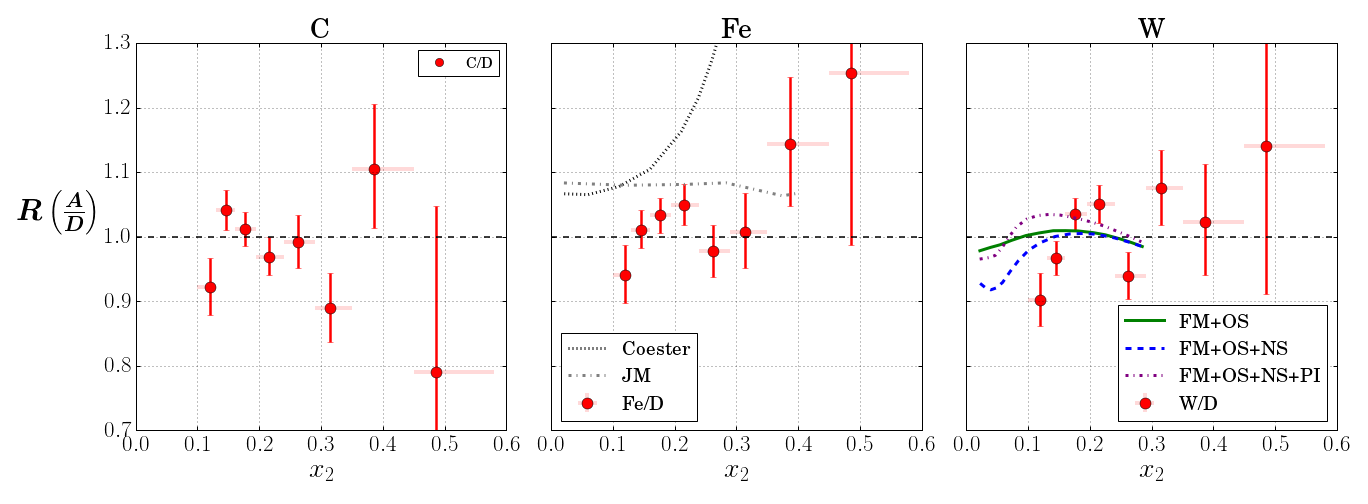
\includegraphics[width=\textwidth]{figures/results/xt-emc-models.png}
	\caption{Some model predictions for DY ratios for $\sigma^{Fe}/\sigma^D$~\cite{Jung:1990pu} and $\sigma^{W}/\sigma^D$~\cite{Kulagin:2015lkm}. All models shown are tuned for \unit[800]{GeV} experiments.}
	\label{fig:xt-emc-models}
\end{figure}

The A-dependent modification of the nucleon has become a challenging and intriguing phenomenon. So many models have arisen attempting to reproduce the data, it has led some of those who study it to give it the moniker \emph{``Every Model is Cool''}~\cite{Miller:1988hj}. Drell-Yan's contributions in isolating particular sea quark components of models' predictions can provide some discriminatory powers between models where DIS data may be satisfied by most models.

% Refer to slides at https://www.jlab.org/intralab/calendar/archive04/pn12/talks/Gaskell.pdf
One particular model is the pion excess model. A proton is not simply three quarks, and a nucleus is not simply a convolution of nucleons. The nucleons themselves are bound by the exchange of mesons at intermediate and long range. These mesons carry a certain fraction of the momentum of the nucleons, and a modification of the meson exchange field in a nuclear medium was predicted by Berger and Coester to lead to an enhancement in the DIS and DY cross section ratios~\cite{Berger:1985dr}. In this model, there is an enhancement in the valence distributions at high $x$, leading to a depletion of valence quarks at intermediate $x$, causing the EMC effect observed.

Seeing as pions carry a valence anti-quark, it was predicted that these intermediary pions would provide an enhancement to the DY cross section ratio for nuclear targets. In Figure~\ref{fig:772-dy}, E-772's DY nuclear cross section ratio results showed strong disagreement with this virtual meson exchange model.

It may, however, be the case that the effect is masked by another effect or the predicted scale is slightly off. In either case, if the pion excess picture is valid, the behavior at higher $x_2$ will still hold and become evident in the SeaQuest data (see predictions by Coester and Jung and Miller for iron in Fig.~\ref{fig:xt-emc-models}). More data at higher $x_2$ will be required to observe if the spike seen in the SeaQuest data for iron and tungsten persist. If so, this could lend support for the Coester view of the pion excess model as, at least in part, contributing to the nuclear modification.

Kulagin and Petti have modeled the composite effects of many nuclear factors such as the pion excess (PI), Fermi motion (FM), off-shell effects (OS), and  nuclear coherence (NS)~\cite{Kulagin:2015lkm} coming together to exhibit the observed behavior of E-772 (see predictions for tungsten in Fig.~\ref{fig:xt-emc-models}). Kulagin and Petti are in contact with SeaQuest and, as of the time of this writing, are preparing a set of predictions for the particular kinematics of SeaQuest. 

%\subsubsection{Rescaling}
%
%In this classification of models, the EMC effect is to be explained by a change in the scale of $Q^2$ used to probe the nucleus as compared to a free nucleon. Alternatively, the momentum fraction $x$ of the probed parton can be scaled commensurately with the size of the nucleus.
%
%In the case of $Q^2$ rescaling, it is explained that~\cite{Rith:2014tma} the strength of the strong force between quarks is ascertained not just by the $1/Q$ at which they are probed, but also by the volume in which they are confined, defined by the nucleon radius $r_A$~\cite{Close:1983tn, Nachtmann:1983py}.  It is therefore relevant to parametrize the strong coupling constant strength not by just $Q^2$, but by $(Q\cdot r_A)^2$.  If the confinement scale is changed for a nucleon inside of a nucleus for any number of reasons, then the parton distributions for nuclei $A$ and $B$ will be related by
%\begin{equation}
%q_A(x,Q^2) = q_B(x,\xi\cdot Q^2)
%\end{equation}
%where $\xi$ is the \emph{rescaling} parameter determined by the nucleus radii (confinement scales) $r_A$ and $r_B$. When considering ``dynamical rescaling'' models, $\xi$ is defined as
%\begin{equation}
%\xi = \left(\frac{r_A}{r_B}\right)^{(2\alpha_s (\mu_A^2))/(\alpha_s(Q^2))}
%\end{equation}
%where $\mu_A$ is a low-momentum cutoff for radiating gluons.
%
%As a result of this $Q^2$ ``dynamical rescaling,'' for the case of $r_A>r_B$ then the structure function ratio $F_2^A/F_2^B>1$ for low $x$ and $F_2^A/F_2^B<1$ for large $x$. A benefit of this model is that it only requires a change in confinement scale of the nucleon, and the mechanism by which this occurs is open ended. Some possible causes could be the ``swelling'' of nucleons, multi-quark ``bags,'' short range correlations, color flow through the nucleus~\cite{Rith:2014tma}, or one of any other model that possibly changes the nucleon confinement scale within a nucleus.
%
%\begin{wrapfigure}{r}{0pt}
%    \centering
%    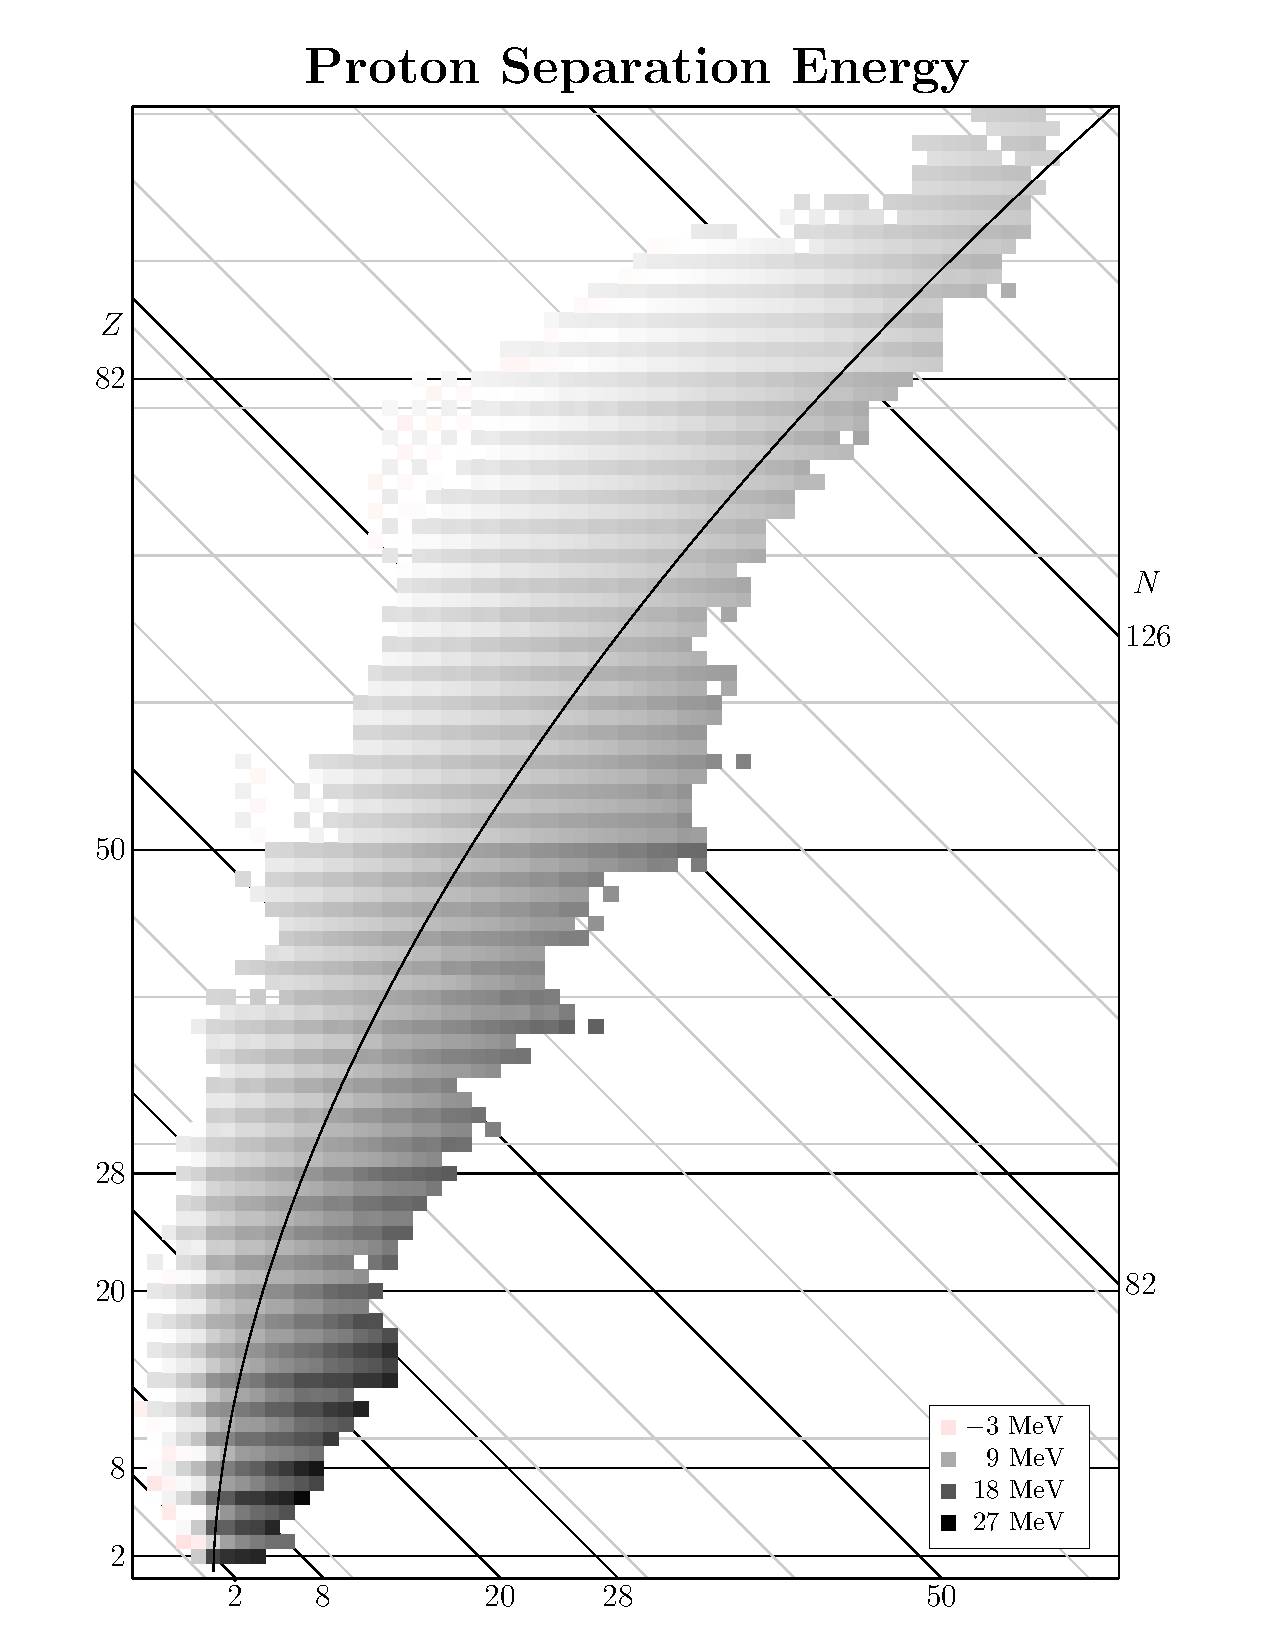
\includegraphics[width=0.35\textwidth]{figures/background/removal-energy.pdf}
%    \caption{The amount of energy required to remove a proton from a nucleus as a function of Z and N~\cite{Dommelen}. This value, $E_i$, is used in the $x$-rescaling model.}
%    \label{fig:nucleon-removal}
%\end{wrapfigure}
%In the case of $x$-rescaling, the EMC effect is explained by nuclear binding and Fermi motion corrections~\cite{GarciaCanal:1984eh, Staszel:1983qx}. In this case, the universal $x$-dependent behavior is explained by x having to be scaled up to a $x_A>x$. In the case of DIS, a nucleon $i$ with momentum $p_i$, the Bjorken-$x$ variable is replaced by:
%\begin{equation}
%x = \frac{Q^2}{2 p_i q} \rightarrow x_A = \frac{Q^2}{2(M+E_i)\nu - 2 \vec{p}_i \vec{q}}
%\end{equation} 
%where $\vec{q}$ is the momentum of the virtual photon and $E_i$ is the removal energy of the nucleon, which can vary between -9 and \unit[-27]{MeV}, depending on the nucleus and whether or not the nucleon in question is a proton or neutron (Fig.~\ref{fig:nucleon-removal}).
%
%As a result of the $x$-rescaling, for the same scattered lepton in DIS, the momentum fraction $x_A$ is probed with regards to the structure function. Since the structure function falls off quickly with increasing $x$, the nuclear structure function ratio depletion is fully explained.
%
%In application, it has been recently discussed by Frankfurt \& Strikman\cite{Frankfurt:2012qs} and implemented by Hen \emph{et al.}\cite{Hen:2013oha} that the \emph{structure functions of nucleons bound in nuclei should be extracted in the reference frame of the nucleus}. This is done by considering to the $x_A$ scaling variable, defined as:
%\begin{equation}
%\frac{x_A}{A} = x_p \cdot \frac{A m_p}{m_A}
%\end{equation}
%where $q$ and $P_A$ are the 4-momentum vectors of the virtual photon and target nucleus respectively, and $m_A$ is the mass of the target nucleus. For the same values of $Q^2$ and $\omega$, $x_A$ differs from $x_p$ by the ratio of the bound nucleon mass to the free mass. Therefore, a cross section measured at $Q^2$ and $\omega$ on a nucleus $A$ will depend on the nucleon structure function evaluated at $x_A$ rather than $x_p$. For converting from the commonly used $x_p$ over to $x_A$ for the different targets, we apply a factor of $\frac{A m_p}{m_A}$, which for deuterium, carbon, iron, and tungsten are AAAAA, BBBBB, CCCCC, and DDDDD, respectively.
%
%As a result, this means that the standard EMC cross section ratio is actually proportional to the nucleon structure function in nucleus $A$ evaluated at parton momentum $x_A$ divided by the nucleon structure function in deuterium evaluated at parton momentum fraction $x_D$ ($x_D = 2Q^2/2m_D\omega = x_p \cdot 2m_p/m_D$)\cite{Hen:2013oha}. For a symmetric nuclei, this can be written as:
%\begin{equation}
%\frac{2}{A} \cdot \frac{\sigma^A_{DY}(x_p, Q^2)}{\sigma^D_{DY}(x_p, Q^2)} = \frac{F_2^A(x_A, Q^2)}{F_2^D(x_D, Q^2)}
%\end{equation}
%where $\frac{F_2^A(x_A, Q^2)}{F_2^D(x_D, Q^2)}$ is the ratio of structure functions at the same $Q^2$, but at different $x$. Since we want to compare the structure functions at the same parton momentum fractions, we correct this by using
%\begin{eqnarray}
%\frac{F_2^A(x_A, Q^2)}{F_2^D(x_D, Q^2)} & = & \frac{F_2^A(x_A, Q^2)}{F_2^D(x_A, Q^2)} \cdot \frac{F_2^D(x_A, Q^2)}{F_2^D(x_D, Q^2)} \\
%& & \nonumber \\
%\frac{F_2^A(x_A, Q^2)}{F_2^D(x_A, Q^2)} & = & \frac{2}{A} \cdot \frac{\sigma^A_{DY}(x_p, Q^2)}{\sigma^D_{DY}(x_p, Q^2)} \cdot \frac{F_2^D(x_D, Q^2)}{F_2^D(x_A, Q^2)}
%\label{eq:struc-func-ratio-xA}
%\end{eqnarray}
%where here we have $\frac{F_2^D(x_D, Q^2)}{F_2^D(x_A, Q^2)}$ as a correction factor to arrive at $\frac{F_2^A(x_A, Q^2)}{F_2^D(x_A, Q^2)}$, which is the ratio of structure functions in the different nuclei evaluated at the same parton momentum fraction (which is what we're looking to extract). The correction factor can be evaluated using well-known parameterizations of the the structure function of the deuteron~\cite{Whitlow:1991uw,Bosted:2007xd}.
%
%In summary, the traditional EMC per-nucleon cross section ratio measurement has yielded a ratio for $\frac{F_2^A(x_A)}{F_2^D(x_D)}$, when what is really desired is $\frac{F_2^A(x_A)}{F_2^D(x_A)}$. The addition of this $\frac{F_2^D(x_D)}{F_2^D(x_A)}$ correction factor is all that is needed to convert the measurement to the desired result. This correction factor will be applied to the SeaQuest result.
